% rubber: module pdftex

\documentclass[a4paper,11pt]{article}
\usepackage[top = 1.5 in, bottom = 1 in, left = 1 in, right = 1 in]{geometry}
\usepackage[utf8]{inputenc}
\usepackage[T1]{fontenc}
\usepackage{csquotes}
\usepackage[british]{babel}
\usepackage{lmodern}
\usepackage{url}
\usepackage{color}
\usepackage{graphicx}
\usepackage{setspace}
\usepackage{pdfpages}
\usepackage{amsmath}

\begin{document}
\title{Compiler project: MiniJava}
\author{Laura Leppänen \\ Compilers, Spring 2012}
\date{\today}
\maketitle
\thispagestyle{empty}

\tableofcontents
\onehalfspacing

\newpage
\setcounter{page}{1}

\section{The Mini-Java language}

\subsection{Token patterns}

Defined using regular expressions with Java style character classes. These token groups correspond to token classes used in the implementation.

\begin{description}
\item[Identifiers] $\backslash\text{p\{IsAlphabetic\}} [ \backslash\text{p\{IsAlphabetic\}}\backslash\text{p\{IsDigit\}\_ } ]^{*}$ \\ \emph{Except simple types and keywords.}
\item[Integer literals] $\backslash\text{p\{IsDigit\}}^{+}$
\item[Simple type] int | boolean | void
\item[Keyword] class | public | static | main | extends | assert | if | else | \\ while | System | out | println | return | new | length | this | true | false
\item[Operator] \&\& | || | < | > | == | + | - | *  | / | \% | = | !
\item[Punctuation] \{ | \} | [ | ] | ( | ) | $\backslash$. | ; | ,
\end{description}

\subsection{Modified grammar for recursive descent parsing (non-LL(1))}

In the grammar below, I have solved operator precedences using the ``classical'' method of making a separate production rule for each level of operator precedence. This is very easy to implement in the case of Mini-Java especially since all the defined binary operators are left-associative and there is only one unary operator. In a more complex case something like the Shunting Yard algorithm would probably work better.\footnote{Note: A program example on the course's grammar page also uses a unary minus operator, but this is not reflected in the grammar that was given, so I have left it out.}

A look-ahead of more than one token is needed e.g. when the parser sees an identifier in the input and is trying to parse a statement. In this case the result could be a local variable declaration for either a user defined type or an array of a user defined type or a statement that starts with an expression that begins with a variable reference.

\begin{verbatim}
<program>              ::= <main class> <class declaration list>
<main class>           ::= "class" <identifier> "{" "public" "static" "void" "main"
                           "(" ")" "{" <statement list> "}" "}"
<class declaration>    ::= "class" <identifier> <optional inheritance> "{"
                           <declaration list> "}"
<optional inheritance> ::= "extends" <identifier>
                        |  epsilon
<declaration>          ::= <variable declaration>
                        |  <method declaration>

<class declaration list> ::= <class declaration> <class declaration list>
                          |  epsilon
<declaration list>       ::= <declaration> <declaration list>
                          |  epsilon
<statement list>         ::= <statement> <statement list>
                          |  epsilon

<method declaration>   ::= "public" <type> <identifier> "(" <opt formals> ")"
                           "{" <statement list> "}"
<opt formals>          ::= <type> <identifier> <formals list>
                        |  epsilon
<formals list>         ::= "," <type> <identifier> <formals list>
                        |  epsilon
<variable declaration> ::= <type> <identifier> ";"
<type>                 ::= <simple type> <opt brackets>
<simple type>          ::= "int" | "boolean" | "void" | <type identifier>
<opt brackets>         ::= "[" "]" | epsilon
<type identifier>      ::= <identifier>

<statement>      ::= "assert" "(" <expr> ")" ";"
                  |  <local variable declaration>
                  |  "{" <statement list> "}"
                  |  "if" "(" <expr> ")" <statement> <opt else>
                  |  "while" "(" <expr> ")" <statement>
                  |  "System" "." "out" "." "println" "(" <expr> ")" ";"
                  |  "return" <expr> ";"
                  |  <expr> <opt assignment> ";"
<opt else>       ::= "else" <statement> | epsilon
<opt assignment> ::= "=" <expr> | epsilon
<local variable declaration> ::= <variable declaration>

<expr> ::= <or-operand> <or-operand-list>
<or-operand> ::= <and-operand> <and-operand-list>
<and-operand> ::= <eq-operand> <eq-operand-list>
<eq-operand>  ::= <neq-operand> <neq-operand-list>
<neq-operand> ::= <add-operand> <add-operand-list>
<add-operand> ::= <mult-operand> <mult-operand-list>
<mult-operand> ::= "!" <term>
                |  <term>

<or-operand-list> ::= "||" <or-operand> <or-operand-list>
                   |  epsilon
<and-operand-list> ::= "&&" <and-operand> <and-operand-list>
                    |  epsilon
<eq-operand-list> ::= "==" <eq-operand> <eq-operand-list>
                   |  epsilon
<neq-operand-list> ::= "<" <neq-operand> <neq-operand-list>
                    |  ">" <neq-operand> <neq-operand-list>
                    |  epsilon
<add-operand-list> ::= "+" <add-operand> <add-operand-list>
                    |  "-" <add-operand> <add-operand-list>
                    |  epsilon
<mult-operand-list> ::= "/" <mult-operand> <mult-operand-list>
                     |  "*" <mult-operand> <mult-operand-list>
                     |  "%" <mult-operand> <mult-operand-list>
                     |  epsilon

<term>    ::= "new" <new type> <opt term tail>
           |  "(" <expr> ")" <opt term tail>
           |  <identifier> <opt term tail>
           |  <integer literal> <opt term tail>
           |  "this" <opt term tail>
           |  "true" <opt term tail>
           |  "false" <opt term tail>

<new type>          ::= <simple type> "[" <expr> "]"
                     |  <type identifier> "(" ")"
<opt term tail>     ::= "[" <expr> "]" <opt term tail>
                     |  "." <method invocation> <opt term tail>
                     |  epsilon
<method invocation> ::= "length"
                     |  <identifier> "(" <opt exprs> ")"
<opt exprs>         ::= <expr list> | epsilon
<expr list>         ::= <expr> <expr list tail>
<expr list tail>    ::= "," <expr list> | epsilon

\end{verbatim}

\newpage

\subsection{Abstract syntax trees}

In this section I describe on an abstract level the interfaces and classes implementing the abstract syntax tree representation and their relationships in the syntax tree.

\subsubsection{An example tree}

The following figure is a partial example of an abstract syntax tree for the sample program with the unary minus eliminated.

\begin{verbatim}
class Factorial {
  public static void main () {
    System.out.println (new Fac ().ComputeFac (10));
  }
}
class Fac {
  public int ComputeFac (int num) {
    assert (num > 0 || num == 0);
    int num_aux;
    if (num == 0)
      num_aux = 1;
    else 
      num_aux = num * this.ComputeFac (num-1);
    return num_aux;
  }
}
\end{verbatim}

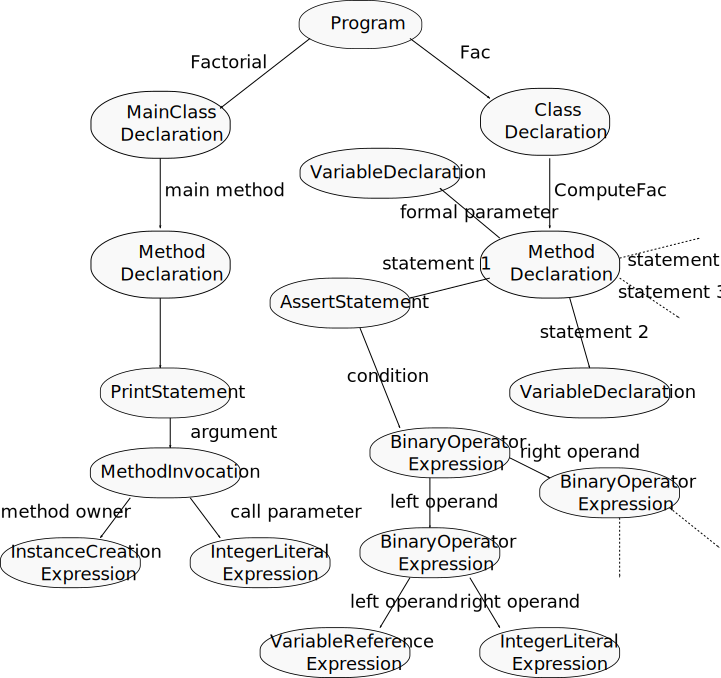
\includegraphics[width=1.0\textwidth]{ast.pdf}

\subsubsection{Interfaces}
\begin{description}
\item[ISyntaxTreeNode] \emph{is a node that can be visited.}
\item[IStatement] \emph{is an} ISyntaxTreeNode \emph{and represents a Mini-Java statement}
\item[IExpression] \emph{is an} ISyntaxTreeNode \emph{and represents a Mini-Java expression}
\end{description}

\subsubsection{Interface implementers}
\begin{description}
\item[Program] \emph{is an} ISyntaxTreeNode \\
\emph{is a root node.} \\
\emph{has a} \textbf{MainClassDeclaration} \\
\emph{has many} \textbf{ClassDeclaration}s
\\
\item[SyntaxElement] \emph{is an abstract} ISyntaxTreeNode \\
\emph{stores row and column information for nodes.}
\\
\item[MainClassDeclaration] \emph{is a} SyntaxElement \\
\emph{has a} \textbf{MethodDeclaration} \emph{which is the main method.} \\
\emph{defines a scope in the semantic analysis phase.}
\item[ClassDeclaration] \emph{is a} SyntaxElement \\
\emph{has many} \textbf{Declaration}s \\
\emph{defines a scope in the semantic analysis phase.}
\\
\item[Declaration] \emph{is an abstract} SyntaxElement \\
\emph{stores type information.}
\item[MethodDeclaration] \emph{is a} Declaration \\
\emph{has many} \textbf{VariableDeclaration}s \emph{which represent formal parameters.} \\
\emph{has many} \textbf{IStatement}s \emph{which form the method body.} \\
\emph{defines a scope in the semantic analysis phase.}
\item[VariableDeclaration] \emph{is a} Declaration \emph{and an} IStatement
\\
\item[AssertStatement] \emph{is a} SyntaxElement \emph{and an} IStatement \\
\emph{has an} \textbf{IExpression} \emph{which is the boolean argument.}
\item[BlockStatement] \emph{is a} SyntaxElement \emph{and an IStatement} \\
\emph{has many} \textbf{IStatement}s \emph{which form the body of the block.} \\
\emph{defines a scope in the semantic analysis phase.}
\item[IfStatement] \emph{is a} SyntaxElement \emph{and an} IStatement \\
\emph{has an} \textbf{IExpression} \emph{which represents the condition.} \\
\emph{has a} \textbf{BlockStatement} \emph{which is the then branch.} \\
\emph{has optionally a} \textbf{BlockStatement} \emph{which is the else branch.}
\item[WhileStatement] \emph{is a} SyntaxElement \emph{and an} IStatement \\
\emph{has an} \textbf{IExpression} \emph{which represents the condition.} \\
\emph{has a} \textbf{BlockStatement} \emph{which is the loop body}
\item[PrintStatement] \emph{is a} SyntaxElement \emph{and an} IStatement \\
\emph{has an} \textbf{IExpression} \emph{which is the integer argument.}
\item[ReturnStatement] \emph{is a} SyntaxElement \emph{and an} IStatement \\
\emph{has an} \textbf{IExpression} \emph{which is the expression to return.}
\item[MethodInvocation] \emph{is a} SyntaxElement \emph{and an} IStatement \emph{and an} IExpression \\
\emph{has an} \textbf{IExpression} \emph{which is the method owner} \\
\emph{has many} \textbf{IExpression}s \emph{which are the call parameters.}
\\
\item[ArrayIndexingExpression] \emph{is a} SyntaxElement \emph{and an} IExpression \\
\emph{has an} \textbf{IExpression} \emph{which is the array reference.} \\
\emph{has an} \textbf{IExpression} \emph{which is the index.}
\item[InstanceCreationExpression] \emph{is a} SyntaxElement \emph{and an} IExpression \\
\emph{has optionally an} \textbf{IExpression} \emph{which is the array size if this is an array creation.} \\
\emph{represents the 'new' expression.}
\item[ThisExpression] \emph{is a} SyntaxElement \emph{and an} IExpression \\
\emph{represents the reference to 'this' class.}
\item[VariableReferenceExpression] \emph{is a} SyntaxElement \emph{and an} IExpression
\item[UnaryOperatorExpression] \emph{is a} SyntaxElement \emph{and an} IExpression \\
\emph{has an} \textbf{IExpression} \emph{which is the operand.}
\item[BinaryOperatorExpression] \emph{is a} SyntaxElement \emph{and an} IExpression \\
\emph{has an} \textbf{IExpression} \emph{that is the left operand.} \\
\emph{has an} \textbf{IExpression} \emph{that is the right operand.}
\item[BooleanLiteralExpression] \emph{is a} SyntaxElement \emph{and an} IExpression
\item[IntegerLiteralExpression] \emph{is a} SyntaxElement \emph{and an} IExpression
\end{description}

\section{Compiler implementation}

This section covers the general architecture of the compiler, testing, error handling as well as the building and running instuctions.

\subsection{Architecture}

The front-end module is divided into three sub-modules, one for each major phase of compilation: lexical analysis, syntax analysis and semantic analysis. In addition, I have collected some things possibly needed by both the front-end and the back-end into the Support module. These include:
\begin{itemize}
\item The abstract syntax tree representation and the related INodeVisitor interface.
\item The symbol table.
\item Static information on the language such as listings of keywords, punctuation characters, operators and operator semantics, precedences etc. This can be expanded to include possible semantic information needed by the back-end later.
\item Error handling: an error reporter interface and a basic implementation for it.
\end{itemize}

\subsubsection{Simplified view of the front-end module}

The FrontEnd class implements the whole front-end compilation pipeline with the help of the aforementioned sub-modules that implement the different phases of compilation. These submodules are descibed starting in the next section.

The idea is to have a separate back-end module that will also have a single class that is parameterised with the output of the front-end phases to bring together the whole back-end pipeline. The whole compiler can then be put together by running these two modules on the program code in succession.

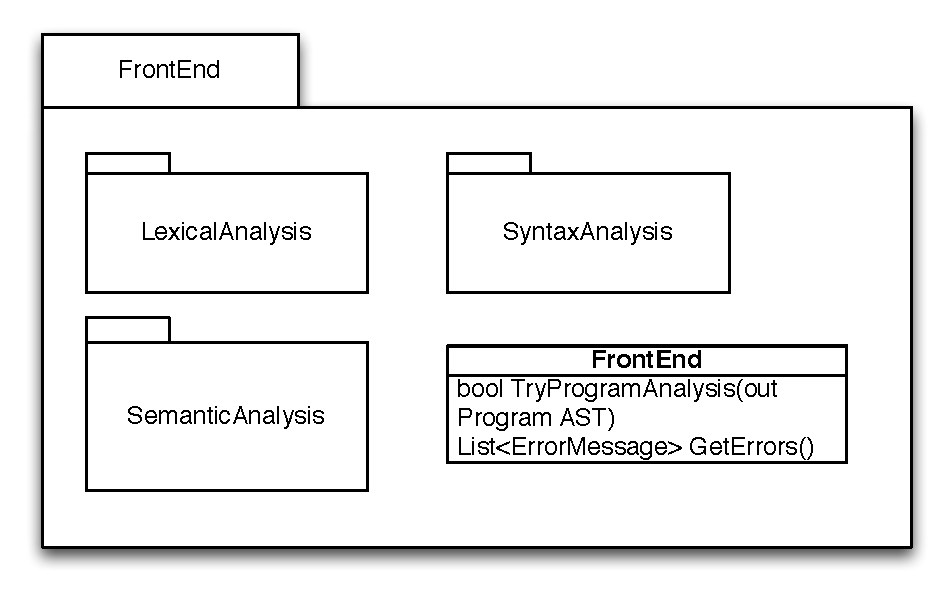
\includegraphics[width=1.0\textwidth]{frontend.pdf}

\subsubsection{Simplified view of the support module}

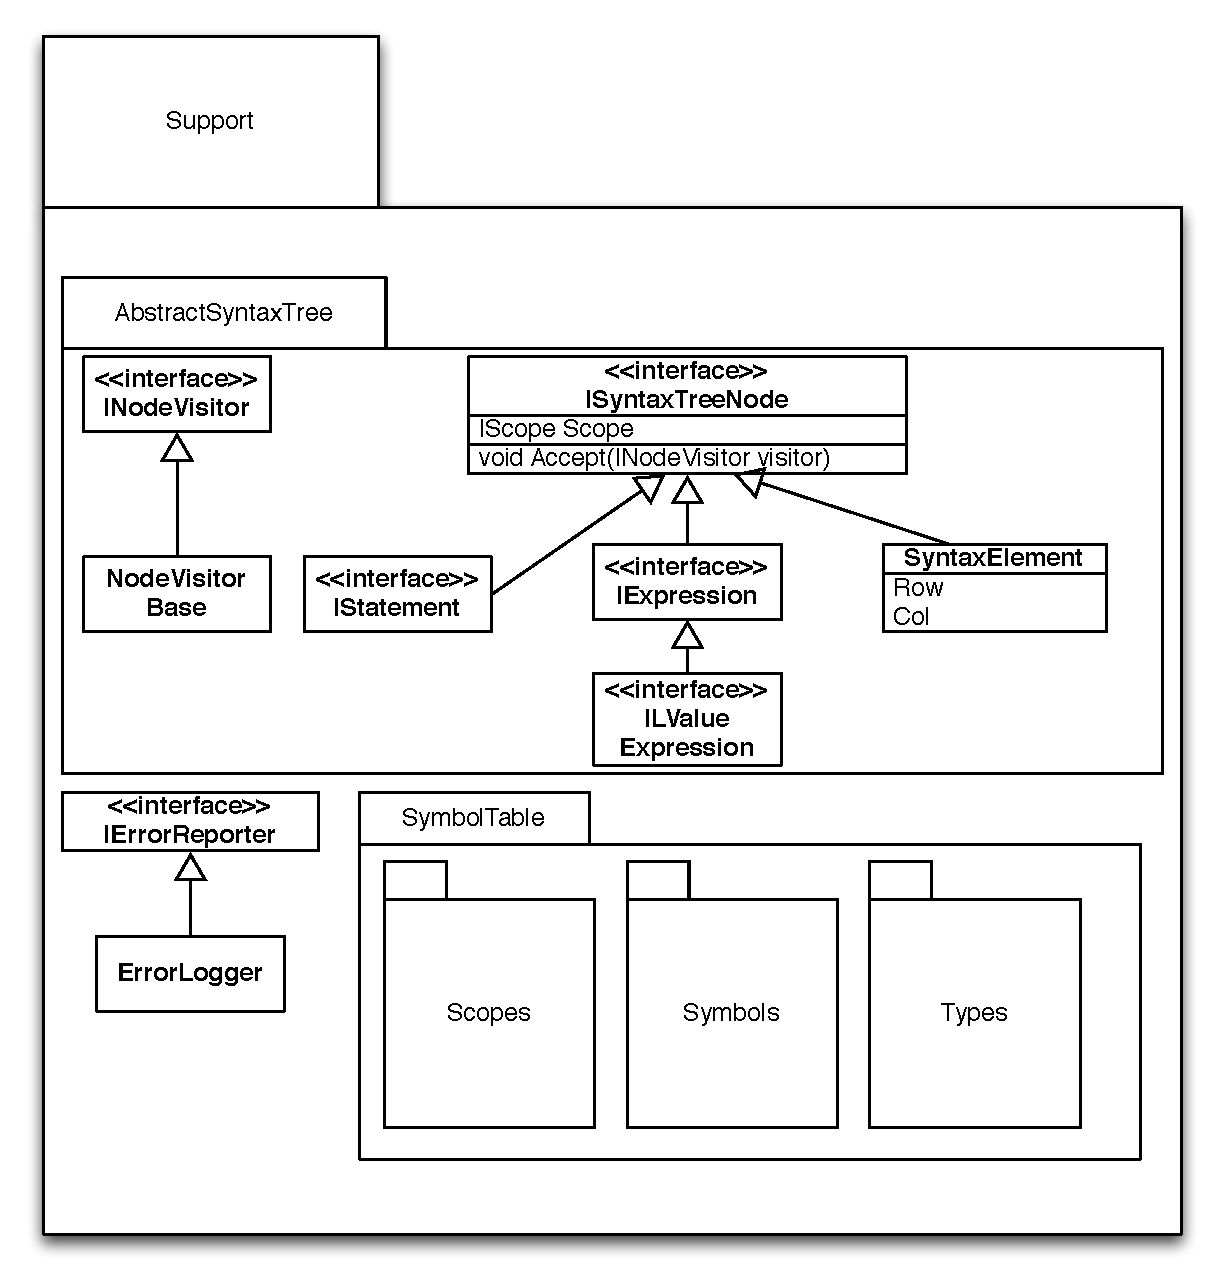
\includegraphics[width=1.0\textwidth]{support.pdf}

\subsection{Lexical analysis}

\subsubsection{Module description}

\begin{figure}[h!]
\centering
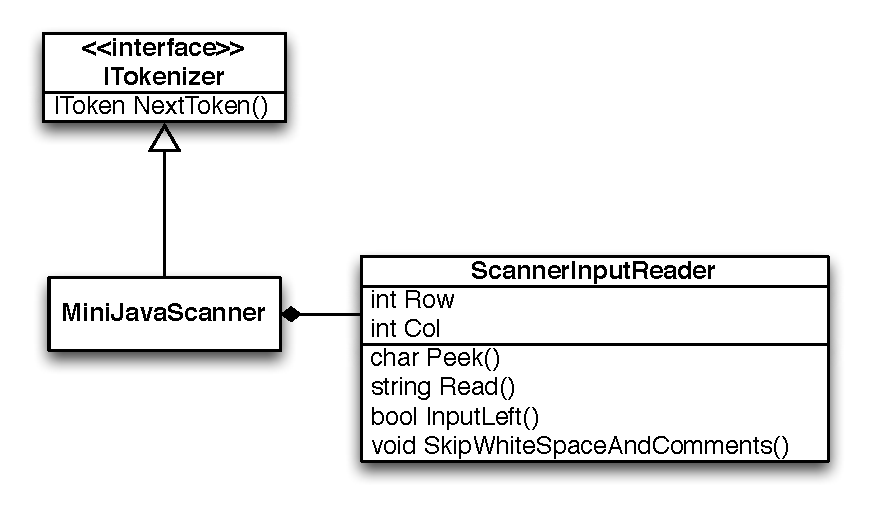
\includegraphics[width=0.7\textwidth]{lexical_analysis.pdf}
\end{figure}

The MiniJavaScanner can read input from either a string or a file: it is parameterised with a TextReader (either a StringReader or a StreamReader) for the program code. It offers a very simple interface: it can be asked for the next token in the input stream. At the end of input, a call to NextToken returns an EndOfFile token. If NextToken is still called after that, an OutOfInput exception will be thrown.

The MiniJavaScanner passes through the code once when instantiated and builds the queue of tokens. This is done so no one can close the TextReader before the whole token stream is ready. The scanner leaves the TextReader open because it is given as a parameter, so it could in theory still be used by the caller.

Internally, the MiniJavaScanner uses a ScannerInputReader to keep track of the current row and column in the input (for error messages), and skip comments and whitespace. This abstracts away all input handling, so the scanner itself stays cleaner and could easily be replaced by another class that would implement the ITokenizer interface.

\subsubsection{Error handling}

The scanner can identify two distinct types of errors:
\begin{enumerate}
\item a multiline comment ended by end of input and
\item an unrecognised token such as characters '\$', '\#' or '@'.
\end{enumerate}

These errors are represented by ErrorToken instances in the token queue. Unlike all other phases of the compiler, the scanner does not throw an exception if it encounters errors like these. The handling of ErrorTokens is left to the caller or the next phase in the pipeline. In practice these errors are handled in the syntax analysis phase.

\subsection{Syntax analysis}

\subsubsection{Module description}

\begin{figure}[h!]
\centering
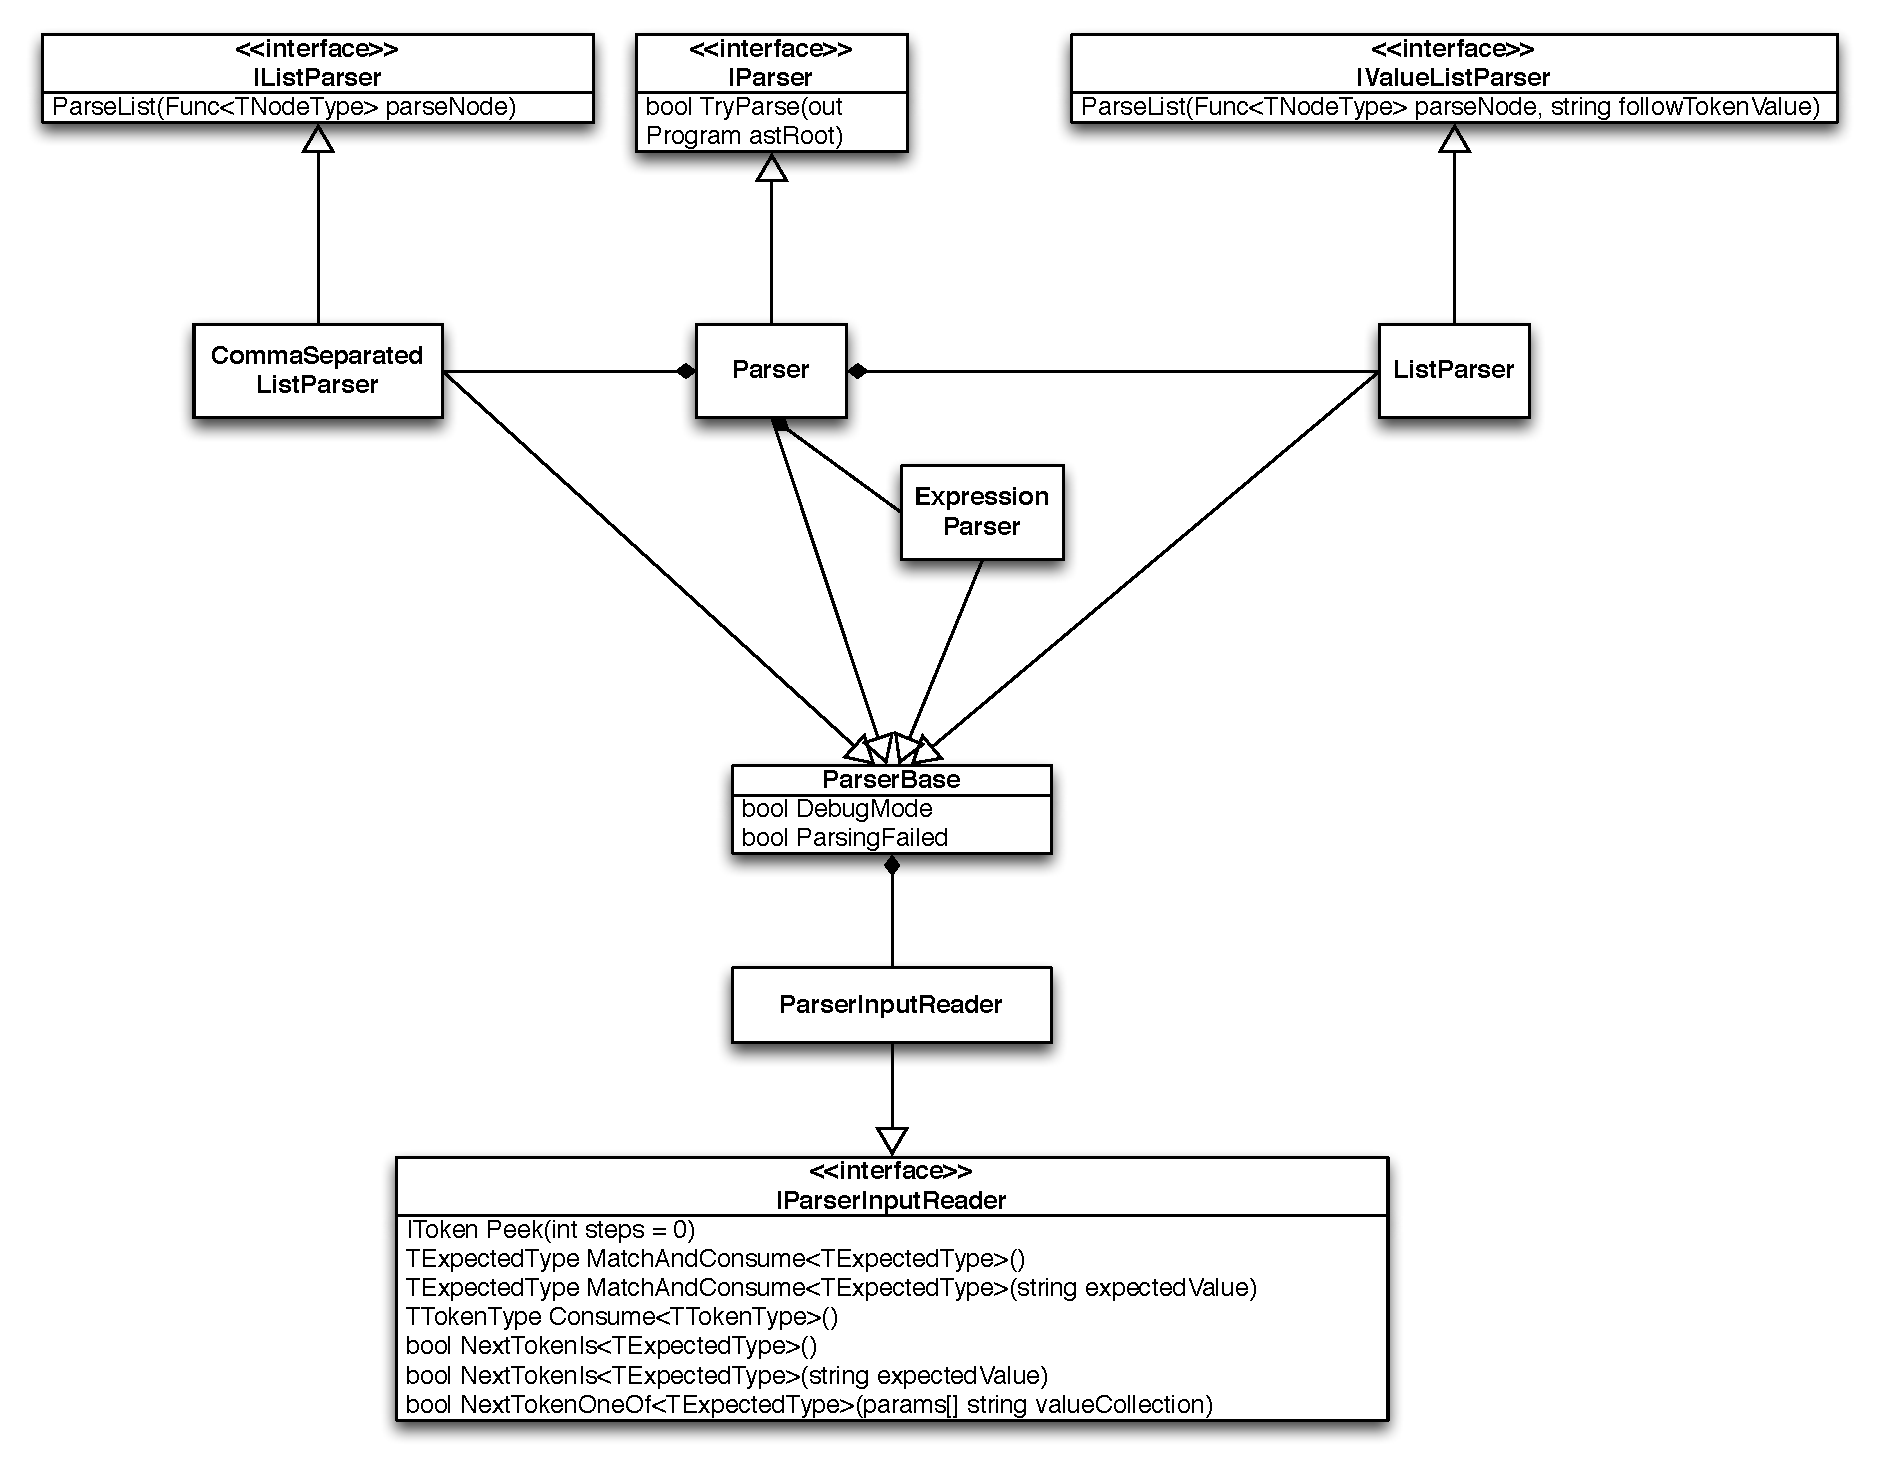
\includegraphics[width=1.0\textwidth]{syntax_analysis.pdf}
\end{figure}

This module is used by instantiating a Parser that takes an ITokenizer an an IErrorReporter as inputs. The error reporter is used to report errors and because it is given as a parameter, a single instance can be shared by several classes and across compilation phases. The default implementation ErrorReporter logs the errors in a list of ErrorMessages which can then be handled by the higher level module that has access to the reporter instance. A custom implementation could e.g. print error messages into standard output in real time when they are reported.

The Parser offers a Parse() method that either returns a Program node (the root of the abstract syntax tree) or throws a CompilationError. In the latter case the list of errors can be accessed through the error reporter. This is the whole interface needed by the caller.

Internally the parser is split into several parts. The main parser creates a new ExpressionParser instance every time it starts parsing an expression. The ExpressionParser takes care of handling e.g. operator precedences using information provided by the MiniJavaInfo support class. This takes some unnecessary complexity out of the main parser class. In theory, the parser could be further split up into e.g. statement and class parsers.

Additionally, there are two list parsers: a generic ListParser that parses nodes with the function parameter until it encounters the end of file or a specified follow set token and a CommaSeparatedListParser that does the same but expects the list to use commas as separators. These are used to parse e.g. parameter and argument lists (comma separated) and lists of classes, statements and declarations.

The parser uses a ParserInputReader (or IParserInputReader) that abstracts away input buffering, peeking (even several steps ahead) and matching tokens to a certain token type and possibly content. The parser can e.g. ask the input reader to check that the next token is a PunctuationToken that has the lexeme '\{', and if so, consume it, cast it to the right type and return it. The Consume method of the ParserInputReader is used every time a token is consumed. If the token consumed is an ErrorToken, the ParserInputReader uses the IErrorReporter to report the error and also informs the actual parser by throwing an appropriate exception. This way all lexical errors get reported.

\subsubsection{Error handling}

The syntax analysis phase can encounter two types of errors:
\begin{enumerate}
\item lexical errors in the form of ErrorTokens from the ITokenizer token queue
\item syntax errors: a token other than what was expected is encountered.
\end{enumerate}

Both types of errors are reported using the IErrorReporter. When an error is encountered, the parser attempts recovery based on reading tokens until one in the follow set is encountered or the end of file is reached. This does not always work terribly well. E.g. if a semicolon is missing from a statement, the recovery routine tries to parse until the next semicolon, because parsing failed while a statement was being parsed. If that statement was the last one in that class, the recovery can end up in the next class.

Expression recovery is especially problematic since the follow set for expressions is large. Some of these problems could possibly be avoided by careful parameterisation of the recovery routines depending on the exact place where a parse error happened but this would make the parser quite a bit more complex and I am not sure whether the exception based error handling used in the current implementation is entirely compatible with these kinds of strategies.

For many common kinds of syntax errors this basic strategy works fine but some pathological cases can cause a stream of uninformative errors following the one actual error\footnote{Examples with explanations can be found in the recovery test code.}. A peculiarity is that often recovery causes an end of input error to be reported twice albeit with two different messages. This is because some methods need to check the type of the input token before choosing the parsing path to take. In this case they can see that the token in the input is an EndOfFile token before any matching is attempted. After this the parser goes into recovery, as is normal when an error is found, and receives an OutOfInput error from the ITokenizer, which causes another reporting of the end of input error.

This peculiarity could easily be fixed by not letting the parsing methods report the error themselves but I have kept this ``feature'' because it produces a bit of useful extra information in some cases.

If no errors are found, parsing ends with the EndOfFile token being consumed and the Program node is returned. If any errors (lexical or syntactic) have been found, a CompilationError is thrown to be handled by the caller.

If syntax analysis fails, the front-end module will not continue compilation into the semantic analysis phase.

\subsection{Semantic analysis}

\subsubsection{Module description}

\begin{figure}[h!]
\centering
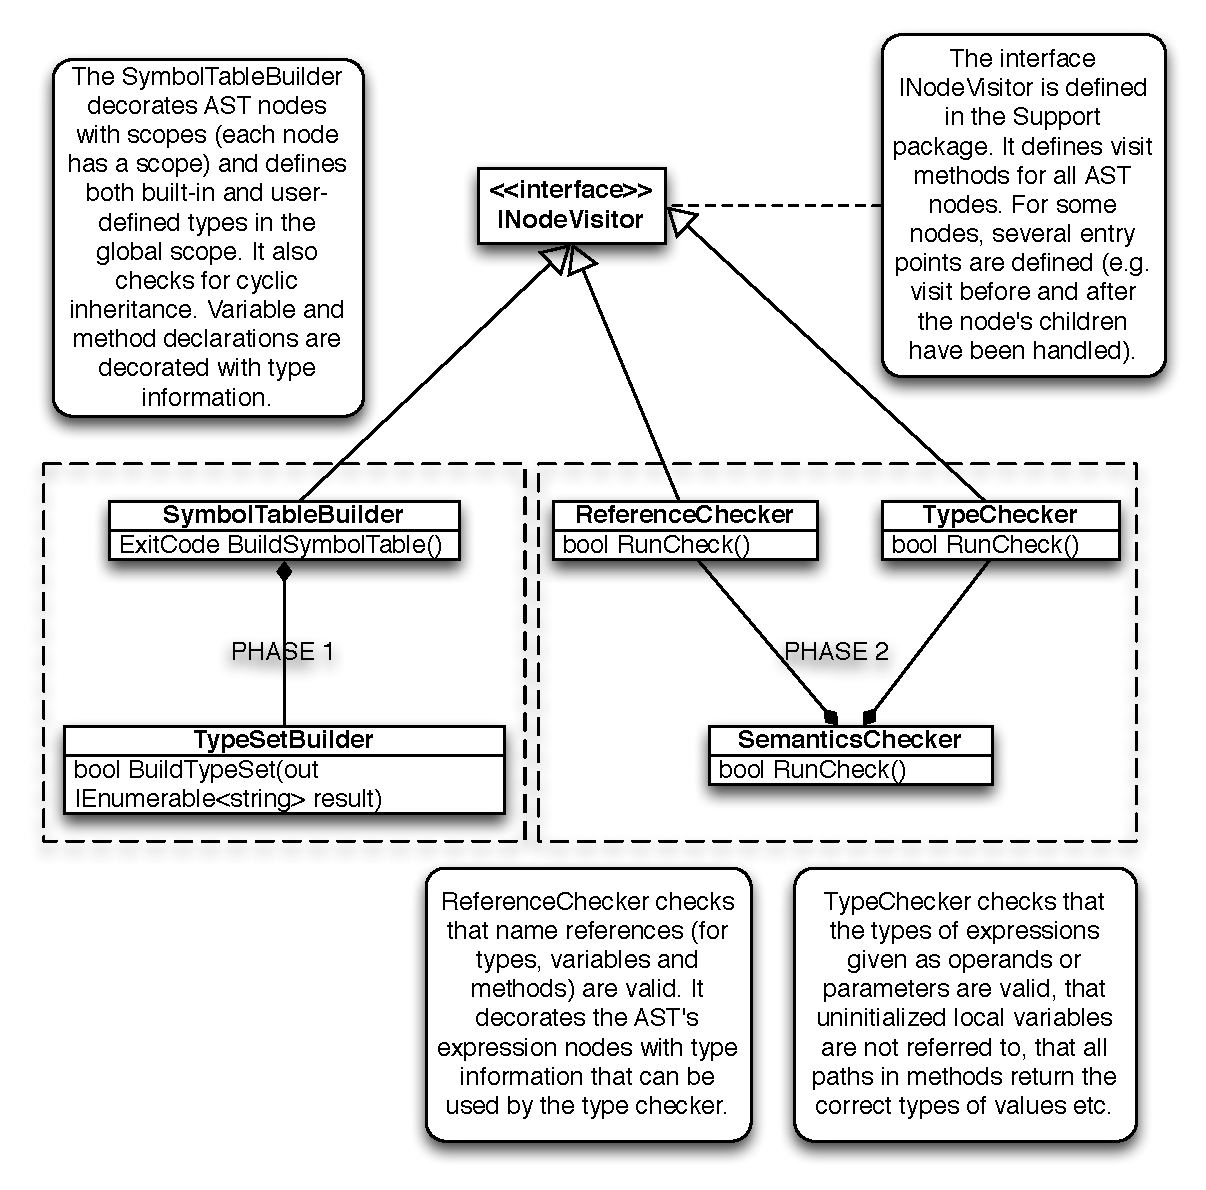
\includegraphics[width=0.8\textwidth]{semantic_analysis.pdf}
\end{figure}

The semantic analysis module is implemented by three classes that are run in succession, each producing input for the next phase. Each internal phase passes once through the abstract syntax tree. The phases are:

\begin{enumerate}
\item Building the set of types (implemented by TypeSetBuilder).
\item Building the symbol table (implemented by SymbolTableBuilder).
\item Checking types and the validity of references (implemented by TypeChecker).
\end{enumerate}

\subsubsection{Building the set of types}

TypeSetBuilder collects all the user defined types (class names) in the program and reports name clashes using an IErrorReporter, again given as a parameter to the constructor. The TypeSetBuilder checks clashes even with built-in types, though this should never happen since having a keyword appear in the place of an identifier would have resulted in a syntax error. If any name clashes are found, a CompilationError is thrown and semantic analysis should not be continued. This module requires no recovery strategies.

\subsubsection{Building the symbol table}

The SymbolTableBuilder requires an IErrorReporter and the list of types built by the TypeSetBuilder. These types as well as all built-in types (int and boolean) are defined in the global scope as the first step. The resulting output is a SymbolTable object which contains the following information:

\begin{itemize}
\item the global scope,
\item a mapping from ISyntaxTreeNodes to IScopes,
\item a mapping from Symbols to ISyntaxTreeNodes (for classes, methods and variable declarations),
\item a type resolver method: all types in Mini-Java can be resolved from the global scope, so this method is provided for convenience,
\item a method to resolve the surrounding class scope for any ISyntaxTreeNode (if one exists).
\end{itemize}

The symbols defined in the symbol table are represented by the following classes which all extend the abstract class Symbol or the derived SimpleTypeSymbol (more on types in the type checking section):

\begin{description}
\item[VariableSymbol] can be defined in an IVariableScope,
\item[BuiltInTypeSymbol] is a concrete SimpleTypeSymbol (Note: void is not defined as a type in the symbol table),
\item[MethodSymbol] is an IVariableScope and can be defined in an IMethodScope,
\item[UserDefinedTypeSymbol] is a concrete SimpleTypeSymbol as well as an IMethodScope and an IVariableScope. It can be defined in an ITypeScope (in Mini-Java this means, in practice, the global scope).
\end{description}

In addition to MethodSymbols and UserDefinedTypeSymbols, there are other IScopes that are not Symbols, namely GlobalScope (an ITypeScope) and LocalScope (an IVariableScope), used for block statements, bodies of conditional statements etc. The bodies of conditional statements have actually been wrapped in BlockStatement nodes in the parsing phase, so they do not need to be handled as special cases when it comes to scoping.

Several types of errors can be detected in this phase:
\begin{enumerate}
\item An attempt to define a symbol when the same type of symbol with the same name is already defined in that scope.
\item A variable or method with an unknown type is declared.
\item A class is declared to be derived from an unknown type.
\end{enumerate}

Same types of symbols from surrounding scopes can be hidden by symbols with the same name, and the same scope can contain e.g. a variable and a method with the same name, so these cases will not result in an error. If an attempt to define a method fails due to a name clash, a LocalScope is instantiated to stand in place of the IMethodScope object that would normally be created, so checks can continue. This is the only recovery strategy required in this phase.

Again, if any errors are encountered, a CompilationError is thrown and further compilation should not be done. Otherwise the phase results in a fully built SymbolTable.

\subsubsection{Checking types and the validity of references}

This phase is implemented by the TypeChecker class. It produces no output in addition to possible errors, again reported using an IErrorReporter instance. A CompilationError is thrown at the end of the check if any errors are found.

This phase can detect the following types of errors:
\begin{enumerate}
\item A method overloads a method in its superclass. Mini-Java allows only overriding, not overloading.
\item If a method overrides a superclass method, the declared return types of the methods are checked. Return type covariance is allowed but anything else results in an error.
\item The arguments to built-in functions or operators (or something similar) are of the wrong type. Examples of these type checks:
\begin{itemize}
\item A print statement requires a single int argument.
\item The argument to an assert statement and the conditional expressions in if and while statements need to be boolean values.
\item Arithmetic operators and comparison operators require two int arguments.
\item Logical binary operators require two boolean arguments and the unary not operator '!' a single boolean argument.
\item Array sizes and indexing expressions must be int values.
\item The equal to operator ('==') accepts any type but both sides must be compatible with each other. Int, boolean and array types require that the other operand is of the same type. For user defined types subtypes are also allowed.
\end{itemize}
\item An attempt is made to index into a variable that is not an array.
\item The left-hand side of an assignment statement is not an L-value. In Mini-Java this means that the left-hand side must be either a reference to a variable (VariableReferenceExpression) or a pointer to an array index (ArrayIndexingExpression).
\item The assigned value in an assignment statement is not compatible with the type of the L-value it is assigned to. The rules are detailed below this error type list.
\item A method invoked for a user defined type cannot be resolved.
\item A method is invoked for a built-in type or an array.\footnote{Note: internally the compiler treats the length property of arrays as a method invocation to avoid having to define it as a special case. This is the only ``method invocation'' allowed for arrays.}
\item A method is invoked with the wrong number of arguments.
\item A wrong type of argument is passed to a method invocation. Type checks for method invocations follow the same rules as type checks for assignment statements, as detailed below.
\item An integer literal is too large to be represented by a 32-bit integer type, which is the only built-in numeric type in Mini-Java.
\item A reference is made to a variable that cannot be resolved or is in the same scope but has not been introduced yet.
\item A void method has return statements. Empty return statements are not defined in the Mini-Java specification, so this is not allowed.
\item At least some paths in a non-void method do not return a value.
\item Return statements return values of a type different from the one declared in the method signature. Again, covariance is allowed, so subtypes of the declared type can be returned.
\item A static method cannot be called on an instance of the defining class. The only static method in Mini-Java is the main method. In my implementation, the main method cannot be called at all because references to the name of the class are not allowed outside type declarations and instance creations. I did not see the reason to implement such a feature since there is no use for calling the main method from inside the program, though the specification is unclear on whether this should be allowed.
\end{enumerate}

The rules for assignment type checking are as follows:
\begin{itemize}
\item An argument of type void cannot be assigned to any L-value.
\item If the L-value is a built-in type, the assigned value must be of the same type. E.g. an index of an int array has type int, so that is the only type of value that can be assigned to it.
\item If the L-value is an array, the assigned value must also be an array and have the same element type. Unlike in Java, covariance of reference types is not allowed here according to the specification given on the course web site.
\item If the L-value is a user defined (reference) type, the assigned value must be the of the same type or a type derived from it.
\end{itemize}

The same rules apply when checking method invocation argument types: just substitute formal parameter type for L-value.

Internally, a type is anything that implements the IType interface. The IType interface requires that the implementer implements a method IsAssignableTo(IType other). BuiltInTypeSymbol and UserDefinedTypeSymbol (both SimpleTypeSymbols) both implement this interface. In addition, there are non-Symbol types: MiniJavaArrayType that is parameterised with a SimpleTypeSymbol (multidimensional arrays are not allowed) and the singleton type VoidType that represents the void return type for methods.

Recovery from errors is needed when the type of an expression cannot be resolved. Type checks are done using an operand type stack, so a placeholder for unresolved types --- the singleton class ErrorType --- is needed. When a method, variable or the type of an instance creation expression cannot be resolved or a non-array variable is indexed, the ErrorType singleton is pushed into the operand stack.

Every IType is required to implement its IsAssignableTo method in such a way, that everything appears to be assignable to an ErrorType -- even the void return type. Similarly, ErrorType is assignable to every other type as well as itself. This way unnecessary type errors related to unresolved types are avoided without having to explicitly check for the ErrorType at every turn. E.g. a program with the line \verb,A foo = new B();, where \verb,B, cannot be resolved results in an error saying that symbol B could not be resolved but not an error saying that an ErrorType cannot be assigned to a variable of type A.

\subsection{Testing}

All modules have been tested using the NUnit test library with a code coverage of nearly 100\%. Only trivial parts have been left untested. Some parts of the program have been unit-tested but most parts should be involved in integration tests.

I have attempted to test the recovery paths in the parsing and semantic analysis phases as well as I could, but thorough testing of recovery routines is very difficult due to the high cyclomatic complexity of recursive parsers and visitors.

The easiest way to run these tests on the department systems with Visual Studio 2010 is to use the NUnit GUI runner, included in the installation package. The NUnit GUI runner cannot, for some reason, be run from a networked drive, so it must be placed in e.g. the user's local home directory.

% TODO: add instructions to actually run the NUnit GUI runner.

An even easier way, if possible, is to install Visual Studio 2012 and use the nuget package manager to install the NUnit framework, because unlike older versions, VS2012 is able to run NUnit tests without any additional test runner plugins. In that case tests can be run straight from the test menu.

\subsection{Building and running the compiler}

The easiest way to build the compiler is probably by opening it in Visual Studio and building it in Release mode to disable assertions and to get optimised code. After this the resulting \verb,MiniJavaCompiler.exe, can be run by giving it the path to the source file as a parameter: \verb,./MiniJavaCompiler.exe path/to/source/file,.

The main program runs the compiler as far as possible, prints error messages or ``Program OK.'' and exits.

\subsection{Possible bugs}

As mentioned in the testing section, the most difficult part of the compiler to test are probably the recovery routines, especially in the parser but to some extent also in the TypeChecker. This is therefore the most likely source of bugs.

If bugs remain in the system (as some almost certainly do), the best case scenario is that they will only lead to bad error messages in some cases. The worst case scenario for the parser is being stuck in an infinite loop when attempting to recover. During development I have found a few such bugs and managed to fix them but I would not be surprised if some untested recovery path still led to such a problem, since the parser is very difficult to reason about.

At the moment, however, I do not know of any existing bugs in the compiler.

The Compiler class that handles file IO and prints out error messages was a last minute addition to make quick tests during e.g. the code review/demo possible, so it may have bugs. The error message handler especially is not very well-tested or robust --- it does not e.g. handle very long lines of code in any special way -- but it should be sufficient for basic hands-on testing if needed.

\appendix
\section{Project definition}

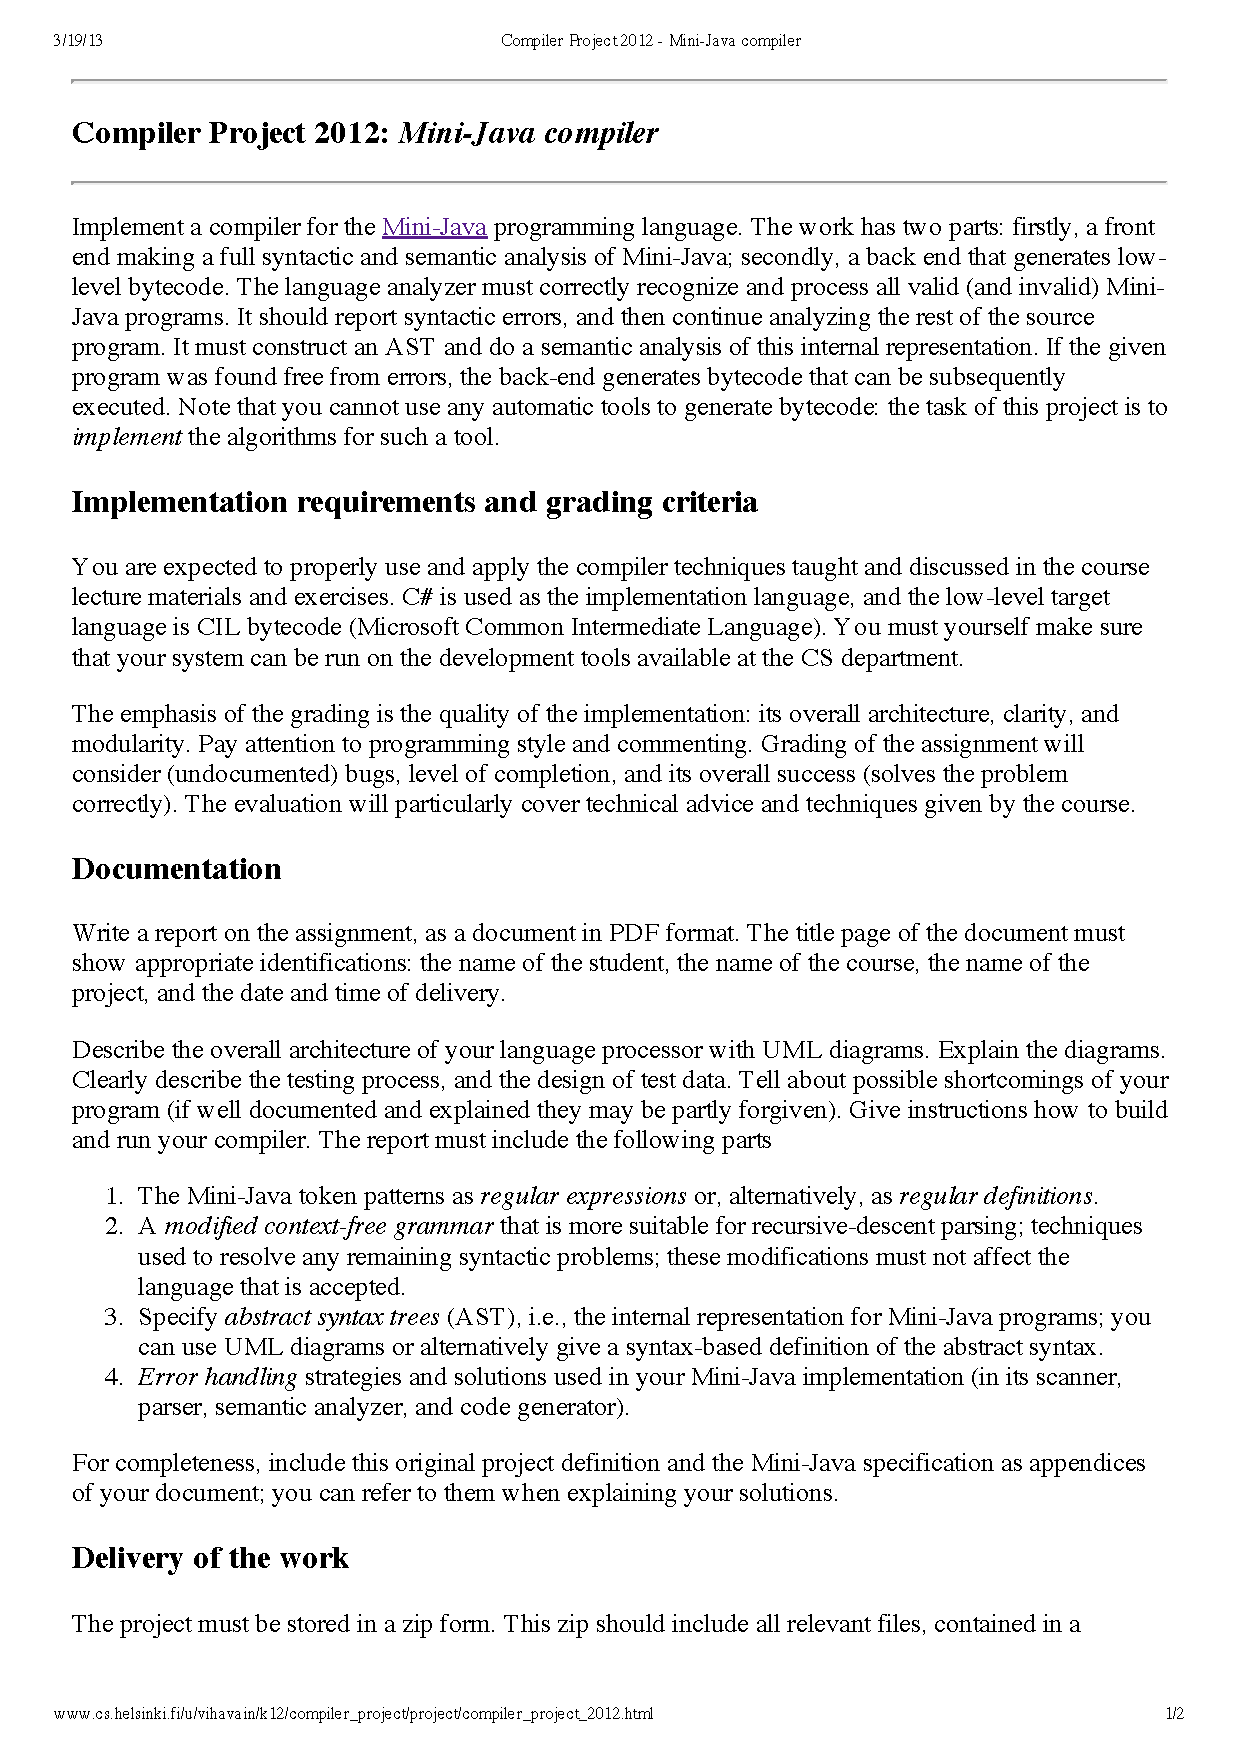
\includegraphics[width=1.0\textwidth,page=1]{project.pdf}
\includegraphics[width=1.0\textwidth,page=2]{project.pdf}

\section{Mini-Java specification}

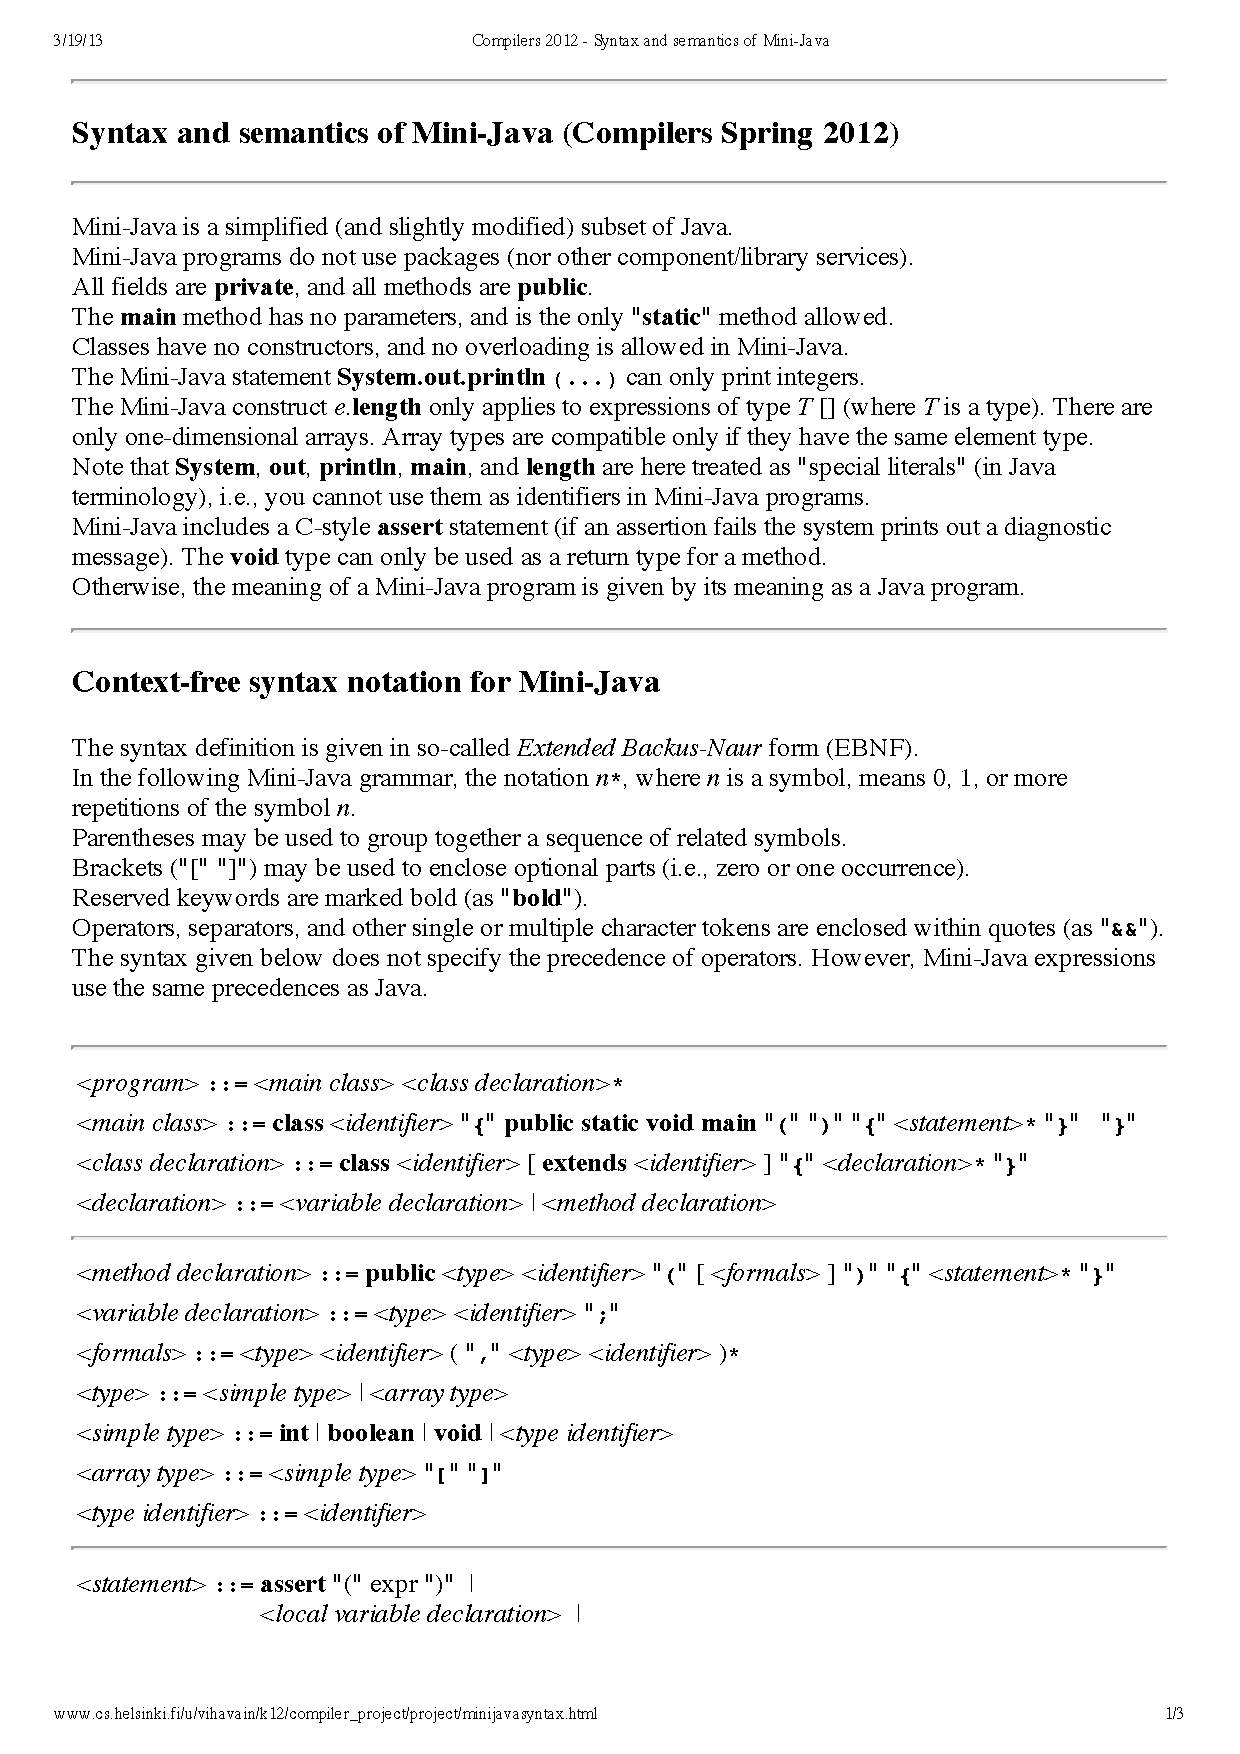
\includegraphics[width=1.0\textwidth,page=1]{spec.pdf}
\includegraphics[width=1.0\textwidth,page=2]{spec.pdf}
\includegraphics[width=1.0\textwidth,page=3]{spec.pdf}
\end{document}
